\documentclass[12pt]{article}

\usepackage{enumerate}
\usepackage{amsmath}
\usepackage{graphicx}
\usepackage{listings}

\setlength\parskip{1em}
\setlength\parindent{0em}

\author{
	Hendrik Werner s4549775
	\and Constantin Blach s4329872
}

\title{Assignment 1}

\begin{document}
\maketitle

\section*{1.1}
The vectors $x, y, z, w, s$ are defined on the exercise sheet.

\subsection*{1.1.1}
\begin{enumerate}[a]
	\item %a
	$v = 3x + y =
	\begin{pmatrix}
		21\\ 28\\ 35\\ 42\\ 49\\ 56\\ 63
	\end{pmatrix}$

	\item %b
	$x \cdotp y = 1057$

	\item %c
	$t = \pi (s + 4) =
	\begin{pmatrix}
		326.72563597\\ 322.95572479\\ 319.1858136\\ 315.41590242\\ 311.64599124
	\end{pmatrix}$

	\item %d
	$z - 1 =
	\begin{pmatrix}
		-.3\\ 0\\ .3\\ .6\\ .9\\ 1.2\\ 1.5\\ 1.8
	\end{pmatrix}$

	\item %e
	We used a loop and Python's feature that you can access a list form the end with negative indexes. After replacing the last 3 values with $4$ we get:

	$x =
	\begin{pmatrix}
		6\\ 7\\ 8\\ 9\\ 4\\ 4\\ 4
	\end{pmatrix}$

	\item %f
	$r = 2w - 5 =
	\begin{pmatrix}
		-3\\ -3\\ -5\\ -4\\ -3\\ -2\\ -1\\ -5\\ -5
	\end{pmatrix}$
\end{enumerate}

\subsection*{1.1.2}
The matrices $M, N, P$ are defined on the exercise sheet.

\begin{enumerate}[a]
	\item %a
	$A = MN + N =
	\begin{pmatrix}
		37 & 19\\
		107 & 59\\
		103 & 56
	\end{pmatrix}$

	\item %b
	$B = N^T * M =
	\begin{pmatrix}
		76 & 99 & 65\\
		24 & 35 & 31
	\end{pmatrix}$

	\item %c
	$C = P^{-1} + P =
	\begin{pmatrix}
		1.66666667 & 5.33333333\\
		5.33333333 & 4.86666667
	\end{pmatrix}$

	Note: It's probably actually
	$\begin{pmatrix}
		\frac{5}{3} & \frac{16}{3}\\
		\frac{16}{3} & 4.86666667
	\end{pmatrix}$
	but because Python uses floating point math we get these results.

	\item %d
	$AC (C + B)$ cannot be computed because $B$ and $C$ have different dimensions. (As do others but one counter example is sufficient.)

	\item %e
	\begin{description}
		\item [$M$]
		The eigenvalues of $M$ are: $14.26208735, -1.26208735, 1$

		The eigenvetors of $M$ are:
		$\begin{pmatrix}
			-0.25759308 & -0.84234218 & 0.51507875
		\end{pmatrix},\\
		\begin{pmatrix}
			-0.68324439 & 0.38109032 & -0.71318597
		\end{pmatrix},\\
		\begin{pmatrix}
			-0.68324439 & 0.38109032 & 0.47545731
		\end{pmatrix}$

		\item [$N$]
		The eigenvalues and eigenvectors of $N$ cannot be computed because $N$ is not square.

		\item [$P$]
		The eigenvalues of $P$ are: $1.72015325, 8.72015325$

		The eigenvetors of $P$ are:
		$\begin{pmatrix}
			-0.80229293 & -0.59693053
		\end{pmatrix},\\
		\begin{pmatrix}
			0.59693053 & -0.80229293
		\end{pmatrix}$
	\end{description}
\end{enumerate}

\section*{1.2}
\subsection*{1.2.1}
\begin{enumerate}[a]
	\item %a
	Firstly we opened the excel file with $open\_workbook$ and opened the first sheet using $sheet\_by\_index$. We created an empty matrix of size 90 by 8 and filled it by iterating over the rows of the excel sheet with an approprioate offset.

	\item %b
	We used pylab to make a scatter plot and show it to the user. This is the plot we got:

	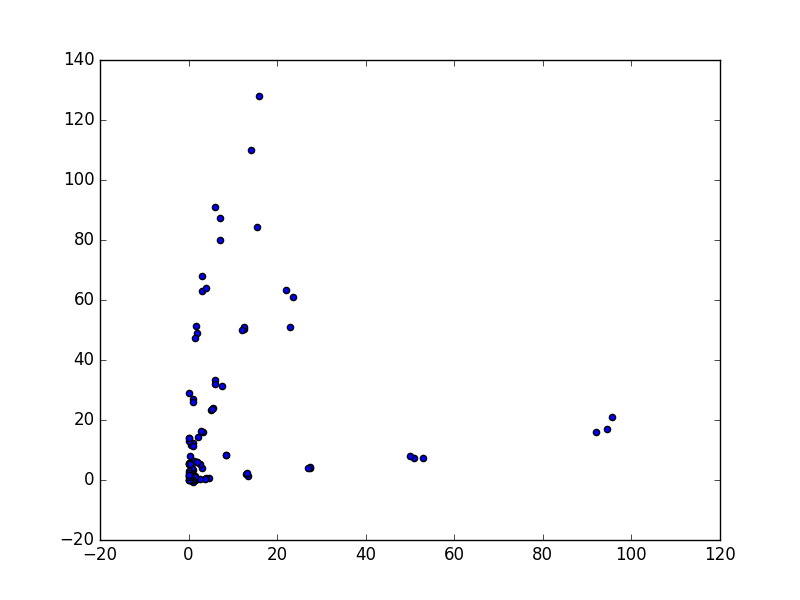
\includegraphics[width=\textwidth]{plot_1_2_1-b}
\end{enumerate}

\subsection*{1.2.2}
\begin{enumerate}[a]
	\item %a
	Principal component analysis (PCA) is a technique that is used to reduce the dimensionality of a data set. The goal is to find the projection that captures the largest amount of variation the the data set.

	The component with the largest variance has the biggest influence on the projection.

	\item %b
	The difference between singular value decomposition (SVD) and eigenvalue decomposition (EVD) is that $\Lambda$ is a diagonal matrix of eigenvalues for EVD and $\Sigma$ is a diagonal matrix of singular values for SVD.

	In SVD the left singular values are eingevectors of $AA^T$ and the right singular values are eigenvectors of $A^TA$ where $A$ is the $m$ by $n$ matrix.

	Because singular values are the squareroot of the eigenvalues SVD and EVD are the same if $A$ is a positive, definite, symmetric matrix.

	\item %c
	The pricipal components of the data set are
	$\begin{pmatrix}
		698.81115865\\ 271.1791264\\ 177.03162195\\ 165.81775197\\ 104.7422797\\ 75.27403086\\ 44.63527635\\ 16.74700977
	\end{pmatrix}$

	The first 3 PCs account for 92.74485381517033\% of the variation. Here is a plot of PCs and their influence in \%:

	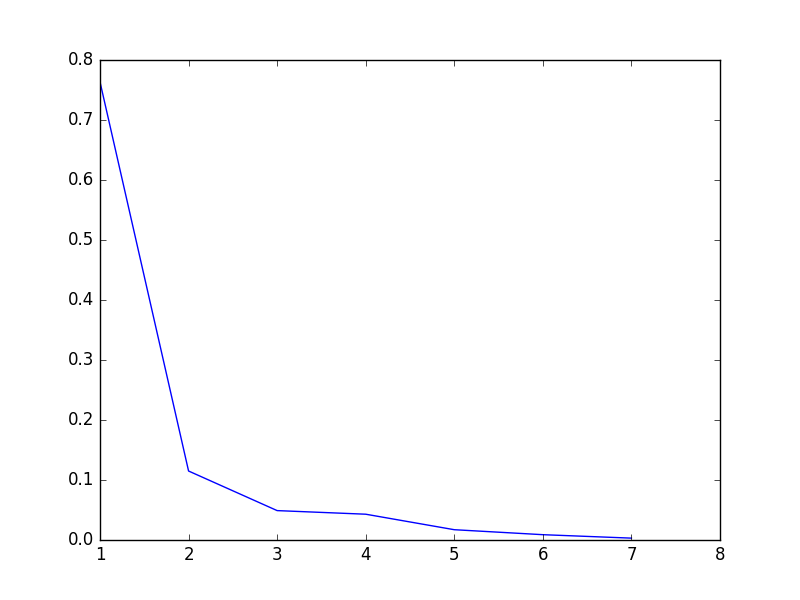
\includegraphics[width=\textwidth]{plot_1_2_2-c}

	\item %d
	We plotted the projections given by the first two PCs against each other:

	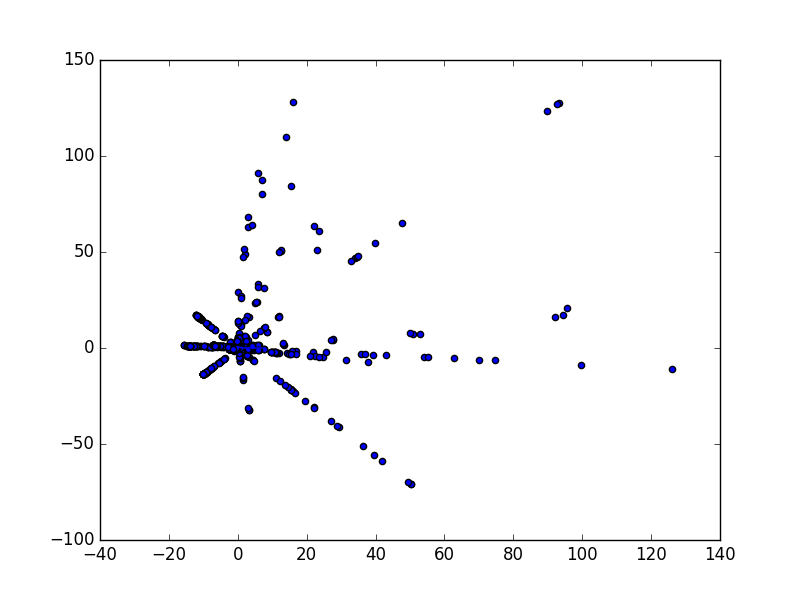
\includegraphics[width=\textwidth]{plot_1_2_2-d}

	This has the advantage that you can now see patterns in the data.

	\item %e
	The PC direction for the second PC is:

	$\begin{pmatrix}
		0.35153606\\ -0.06817937\\ 0.16197185\\ 0.16124192\\ -0.749146\\ -0.37473452\\ -0.31953982\\ -0.1256533
	\end{pmatrix}$

	Attribute E has the biggest influence on this projection.
\end{enumerate}

\section*{1.3}
\subsection*{1.3.2}
We tried using this code to test similarity:

\begin{lstlisting}
import numpy
import scipy

v1 = numpy.array([14, 22, 13, 44, 25])
v2 = numpy.array([41, 5, 1, 3, 5])

print(scipy.spatial.distance.cosine(5 * v1, v2)
      == scipy.spatial.distance.cosine(v1, v2))
\end{lstlisting}

but we got this error:

\begin{lstlisting}
AttributeError: module 'scipy' has no attribute 'spatial'
\end{lstlisting}

We did not know how to solve this.
\end{document}
